\documentclass{beamer}
\usepackage[titlepage=images/titlepage.jpg]{uibkstyle}
\usepackage[utf8]{inputenc}
\usepackage[german]{babel}
\usepackage{graphicx}
\usepackage{subfigure}

\usepackage{tikz}
\usetikzlibrary{decorations.pathmorphing}

\graphicspath{{images/}}

\tikzset{
    onslide/.code args={<#1>#2}{%
        \only<#1>{\pgfkeysalso{#2}}
    },
    month/.style={%
        text depth=.25ex,
        text centered,
    }
}
\tikzset{
    other/.style={circle, onslide=<3-7>{white}}
}

\usetikzlibrary{positioning, arrows, decorations.markings}
\tikzset{%label colors for port states
    port/.style={draw, circle},
    dedicated/.style={port, fill=blue!50},
    root/.style={port, fill=green!50},
    blocking/.style={port, fill=red!50}
}

\tikzset{%used for "invisible" stuff
    invisible/.style={draw=white}
    visible/.style={draw=black}
}

\newcommand{\switch}[2]{
    \scalebox{#1}{
        \begin{tikzpicture}
            \node at (0,0) {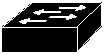
\includegraphics{switch.pdf}};
            \node at (0,-0.6) {#2};
        \end{tikzpicture}
    }
}


\title{STPViz}
\subtitle{Visualizing network topologies with the help of the Spanning Tree Protocol}
\author{Alexander Schlögl}

\begin{document}
\begin{frame}[plain]
    \maketitle
\end{frame}

\begin{frame}{Überblick}
    \begin{itemize}
        \item \textbf{Spanning Tree Protocol (STP)}
        \item \textbf{Kommerzielle Tools}
        \item \textbf{STPViz}
        \item \textbf{Konklusion}
    \end{itemize}
\end{frame}

\begin{frame}{Warum STP?}
    \centering
    \begin{figure}
        \begin{tikzpicture}
            \node (root) at (4,8) {\switch{0.8}{A}};
            \node (B) at (2,6) {\switch{0.8}{B}};
            \node (C) at (6,6) {\switch{0.8}{C}};
            \node (D) at (4,4) {\switch{0.8}{D}};

            \draw
            [onslide=<2>{green, thick, ->},
            onslide=<4>{green,thick, <-},
            onslide=<5>{red,thick,<->}]
            (root) edge (B);

            \draw
            [onslide=<2>{green, thick, ->},
            onslide=<4>{green,thick, <-},
            onslide=<5>{red,thick,<->}]
            (root) edge (C);

            \draw
            [onslide=<3>{red, thick, <->},
            onslide=<5>{red, thick, <->}]
            (B) edge (C);

            \draw
            [onslide=<3>{green, thick, ->},
            onslide=<4-5>{red,thick,<->}]
            (B) edge (D);

            \draw
            [onslide=<3>{green, thick, ->},
            onslide=<4-5>{red,thick,<->}]
            (C) edge (D);
        \end{tikzpicture}
    \end{figure}
\end{frame}

\begin{frame}{Broadcasts mit STP}
    STP deaktiviert doppelte Verbindungen zur Root.\\
    Baumtopologie entsteht.
    \pause
    \begin{figure}
        \begin{tikzpicture}
            \node (root) at (4,8) {\switch{0.8}{A}};
            \node (B) at (2,6) {\switch{0.8}{B}};
            \node (C) at (6,6) {\switch{0.8}{C}};
            \node (D) at (4,4) {\switch{0.8}{D}};

            \draw
            [onslide=<+(1)>{green,thick,->}]
            (root) edge (B);

            \draw
            [onslide=<.(1)>{green,thick,->}]
            (root) edge (C);

            \draw
            [onslide=<+(1)>{green,thick,->}]
            (B) edge (D);
        \end{tikzpicture}
    \end{figure}
\end{frame}

\begin{frame}{Problemstellung}
    \begin{itemize}[<+->]
        \item Große Netzwerke sind schwer zu administrieren
        \item STP verbirgt Fehler und Änderungen zusätzlich
        \item STP Konfiguration ist komplex
    \end{itemize}
    \pause
    Kommerzielle Tools existieren.\\
    \alert{Aber: Diese nutzen SNMP}
\end{frame}

\begin{frame}{SNMP}
    \centering
    \begin{figure}
        \begin{tikzpicture}
            \node (root) at (4,8) {\switch{0.8}{A}};
            \node (B) at (2,6) {\switch{0.8}{B}};
            \node (C) at (6,6) {\switch{0.8}{C}};
            \node (D) at (4,4) {\switch{0.8}{D}};

            \node (PC) at (6.5,3.5) {Client};

            \draw
            (root) -- (B)
            (root) -- (C)
            (B) -- (D);

            \draw[onslide=<1>{white},onslide=<2>{pantone289,thick,->},onslide=<3>{pantone289,thick,<-}]
            (PC) edge (root)
            (PC) edge (B)
            (PC) edge (C)
            (PC) edge (D);
        \end{tikzpicture}
    \end{figure}
\end{frame}

\begin{frame}{STPViz}
    \centering
    \begin{figure}
        \begin{tikzpicture}
            \node (root) at (4,8) {\switch{0.8}{A}};
            \node (B) at (2,6) {\switch{0.8}{B}};
            \node (C) at (6,6) {\switch{0.8}{C}};
            \node (nc) at (7, 4.5) {Client};
            \node (D) at (4,4) {\switch{0.8}{D}};
            \node (nd) at (2.5, 2.5) {Client};
            \node (s) at (5.5, 2.5) {Server};

            \draw
            (root) -- (B)
            (root) -- (C)
            (B) -- (D)
            (C) -- (nc)
            (D) -- (nd);

            \draw[pantone289, thick, ->]
            (nc) edge (s)
            (nd) edge (s);
        \end{tikzpicture}
    \end{figure}
\end{frame}

\begin{frame}{STP Pakete}
    \centering
    \begin{figure}
        \begin{tikzpicture}[scale=0.35]
            \foreach \x in {0,...,31}
            \node at (\x+0.5,20.5) {\scriptsize \x};
            \draw (0,20) rectangle (16,18.5); \node (mode) at (8, 19.25) {Protocol Identifier};
            \draw (16,20) rectangle (24,18.5); \node (mode) at (20, 19.25) {Version Id};
            \draw (24,20) rectangle (32,18.5); \node (mode) at (28, 19.25) {BPDU Type};
            \draw (0,18.5) rectangle (8,17); \node (mode) at (4, 17.75) {Flags};
            \draw[red, line width=2pt] (8,18.5) rectangle (32,17); \node (mode) at (20, 17.75) {Root Identifier};
            \draw[red, line width=2pt] (0,17) rectangle (32,15.5); \node (mode) at (16, 16.25) {Root Identifier};
            \draw[red, line width=2pt] (0,15.5) rectangle (8,14); \node (mode) at (4, 14.75) {Root Identifier};
            \draw (8,15.5) rectangle (32,14); \node (mode) at (20, 14.75) {Root Path Cost};
            \draw (0,14) rectangle (8,12.5); \node (mode) at (4, 13.25) {Root Path Cost};
            \draw[blue, line width=2pt] (8,14) rectangle (32,12.5); \node (mode) at (20, 13.25) {Bridge Identifier};
            \draw[blue, line width=2pt] (0,12.5) rectangle (32,11); \node (mode) at (16, 11.75) {Bridge Identifier};
            \draw[blue, line width=2pt] (0,11) rectangle (8,9.5); \node (mode) at (4, 10.25) {Bridge Identifier};
            \draw (8,11) rectangle (24,9.5); \node (mode) at (16, 10.25) {Port Identifier};
            \draw[green, line width=2pt] (24,11) rectangle (32,9.5); \node (mode) at (28, 10.25) {Message Age};
            \draw[green, line width=2pt] (0,9.5) rectangle (8,8); \node (mode) at (4, 8.75) {Message Age};
            \draw (8,9.5) rectangle (24,8); \node (mode) at (16, 8.75) {Max Age};
            \draw (24,11) rectangle (32,8); \node (mode) at (28, 8.75) {Hello Time};
            \draw (0,8) rectangle (8,6.5); \node (mode) at (4, 7.25) {Hello Time};
            \draw (8,8) rectangle (24,6.5); \node (mode) at (16, 7.25) {Forward Delay};
        \end{tikzpicture}
    \end{figure}
\end{frame}

\begin{frame}{Pfadkonstruktion}
    \centering
    \begin{figure}
        \begin{tikzpicture}
            \node (A) at (4,8) {\switch{0.8}{A}};
            \node (B) at (2,6) {\switch{0.8}{B}};
            \node (C) at (6,6) {\switch{0.8}{C}};
            \node (D) at (4,4) {\switch{0.8}{D}};
            \node (cd) at (4,2) {Client};

            \draw[green, thick]
            (cd) -- (D);

            \draw[white,onslide=<2->{green, thick}]
            (D) -- (B);
            \draw[white, onslide=<3>{green, thick}]
            (A) -- (B);
            \draw[onslide=<1-2>{white}]
            (A) -- (C);
        \end{tikzpicture}
    \end{figure}
\end{frame}

\begin{frame}{Problem}
    \begin{figure}[h]
        \begin{tikzpicture}
            \node (A) at (4,8) {\switch{0.8}{A}};
            \node (B) at (2,6) {\switch{0.8}{B}};
            \node (C) at (6,6) {\switch{0.8}{C}};
            \node (D) at (4,4) {\switch{0.8}{D}};
            \node (client) at (4,2) {Client};

            \draw
            (C) -- (D);

            \draw[white, onslide=<2>{black}]
            (A) -- (C);

            \draw[green, thick, onslide=<2>{red}]
            (B) --  (D)
            (D) --  (client);

            \draw[white, thick, onslide=<2>{red, dashed}]
            (A) -- (B);

        \end{tikzpicture}
    \end{figure}
\end{frame}

\begin{frame}{Fehlerkorrektur}
    \begin{figure}
        \begin{tikzpicture}
            \node (A) at (4,8) {\switch{0.8}{A:0}};
            \node (C) at (6,6) {\switch{0.8}{C:1}};
            \node (D) at (4,4) {\switch{0.8}{D:2}};
            \node (client) at (4,2) {Client};

            \node (B) at (2,6) {
                \scalebox{0.8}{
                    \begin{tikzpicture}
                        \node at (0,0) {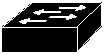
\includegraphics{switch.pdf}};
                        \node[onslide=<2->{white,opacity=0}] at (0,-0.6){B:1};
                        \node[onslide=<1>{white,opacity=0}] at (0,-0.6){\alert{B:3}};
                    \end{tikzpicture}
                }
            };

            \draw
            (A) -- (C)
            (C) -- (D)
            (B) -- (D)
            (D) -- (client);

            \draw [red, thick, dashed, onslide=<2->{white}]
            (A) -- (B);
        \end{tikzpicture}
    \end{figure}
\end{frame}

\begin{frame}{Konklusion}
    Was wurde erreicht?
    \only<3>{
        \vspace{0.5cm}
        \begin{center}
            \scalebox{0.9}{
                \begin{tikzpicture}[]
\node (0) at (7.000000,20) {32768:0 - BC:AE:C5:EB:7D:B6, 0};
\node (1) at (3.500000,18) {32768:1 - 00:E0:7C:C8:57:E7, 1};
\node (2) at (3.500000,16) {61440:0 - F4:F2:6D:7D:BF:BD, 2};
\draw 
(1) -- (2);
\node (3) at (10.500000,18) {32768:1 - 00:E1:00:00:0D:C4, 1};
\draw 
(0) -- (1)
(0) -- (3);
\end{tikzpicture}

            }
        \end{center}
    }
    \onslide<2>{
        \begin{figure}
            \centering
            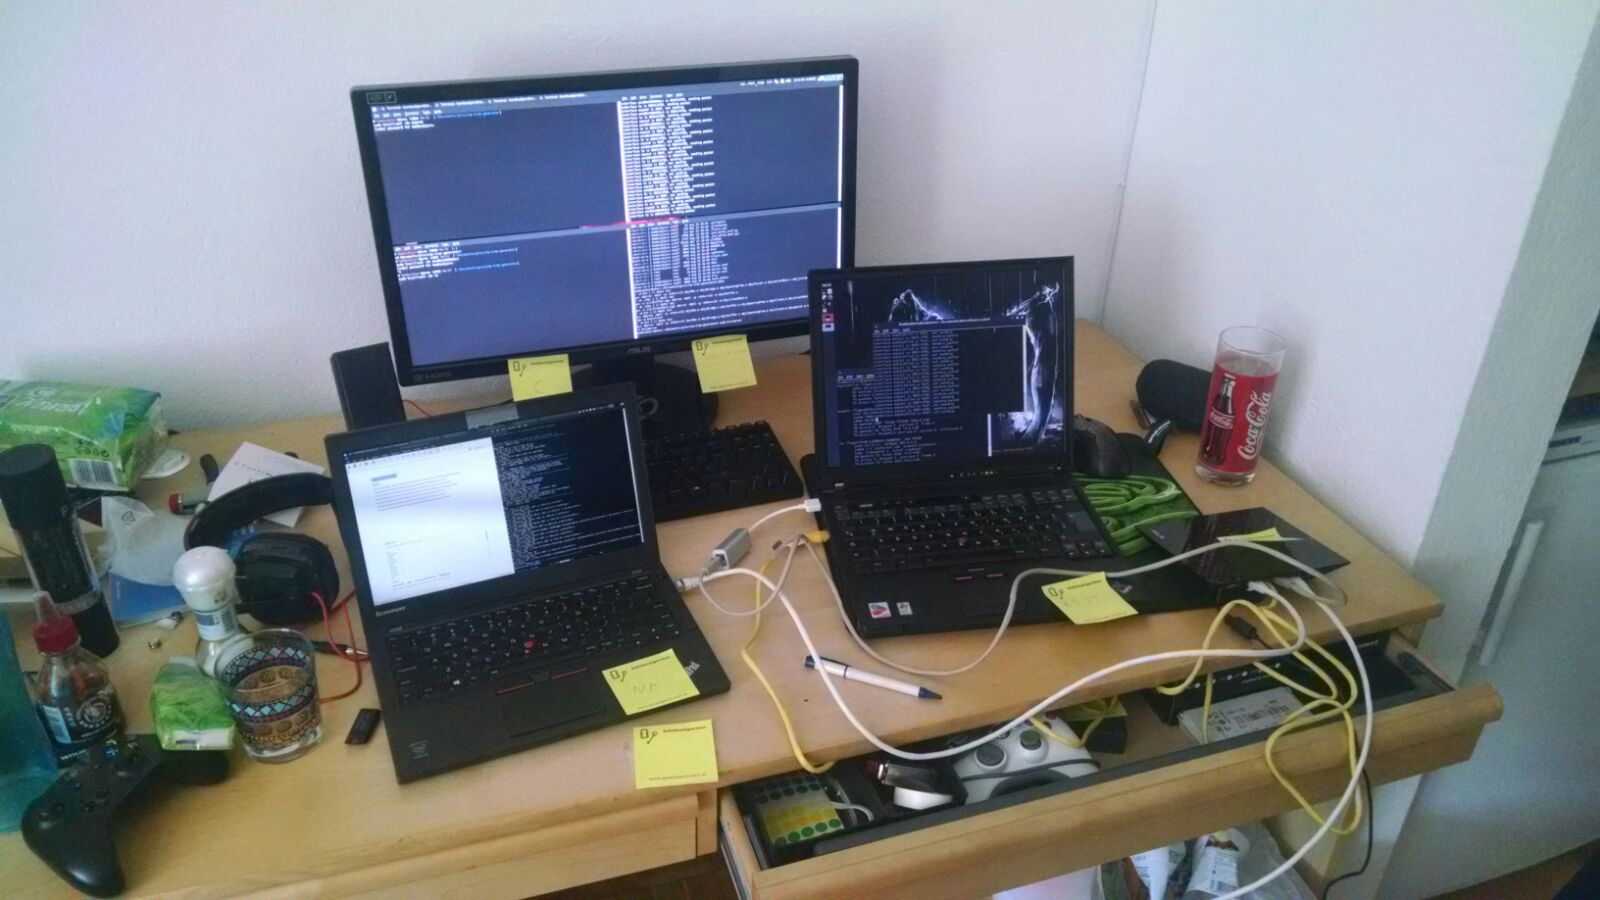
\includegraphics[width=\textwidth]{physicalSetup.jpg}
        \end{figure}
    }
\end{frame}

\begin{frame}{Konklusion}
    In Worten:
    \begin{itemize}[<+(1)->]
        \item Visualisierung nur mit STP sehr schwer
        \item STPViz schafft dies mit Annahmen
        \item Fehlerkorrektur mit $\mathcal{O}(n^2)$ Komplexität
        \item Weniger mächtig als kommerzielle Tools, setzt aber weniger vorraus
    \end{itemize}
    \onslide<7>{\alert{STPViz bietet eine Grundlage für zukünftige mächtigere Tools}}
\end{frame}

\end{document}
